\documentclass[pdf]{beamer}
\usepackage[english,vietnamese]{babel}
\usepackage{amsmath}
\usepackage{booktabs}
\usepackage{graphicx}
\usepackage{hyperref}
\usepackage{lmodern}
\usepackage{siunitx}

\mode<presentation>{}
\usetheme[hideothersubsections]{Hannover}
\usefonttheme[onlymath]{serif}
\usebackgroundtemplate{
  
\includegraphics[width=\paperwidth,height=\paperheight]{USTH.jpg}}
\renewcommand{\thefootnote}{\fnsymbol{footnote}}
\setcounter{tocdepth}{2}

\title[RECIPE]{Random Experiments on Color Image Processing and Enhancement}
\author[Group 8]{Trần Minh Hiếu---BI9-101\\
                 Nguyễn Gia Phong---BI9-184\\
                 Nguyễn Văn Tùng---BI9-229\\
                 Nguyễn An Thiết---BI8-174\\
                 Nguyễn Thành Vinh---BI8-187}
\institute{University of Science and Technology of Hà Nội}
\date{\selectlanguage{english}\today}

\begin{document}
\frame{\titlepage}
\selectlanguage{english}
\section{Introduction}
\begin{frame}{Contents}
  \tableofcontents
\end{frame}
\begin{frame}{Humans and Colors}
  \begin{itemize}\Large
    \item Humans see the world in color
    \item Humans \emph{love} colors!
    \item Color paintings, color pictures, color movies
  \end{itemize}
\end{frame}

\begin{frame}{Colors Image Processing}\Large
  \begin{itemize}
    \item Most techniques similar to\\
      that of monochrome images
    \item There exists color-image-specific stuff too!
    \item And how computers represent colors?
  \end{itemize}
\end{frame}

\section{Color Spaces}
\frame{\tableofcontents[currentsection]}
\begin{frame}{Why So Many?}\Large
  \begin{itemize}
    \item Each usage is needs a different color space
    \item Examples: RGB for computer display,\\
      CMYK for printing
    \item People try to standardize color specifications
    \item And people often don't agree,\\
      e.g. HSV vs HSB vs HSL
  \end{itemize}
\end{frame}

\begin{frame}{Relevant xkcd}
\begin{center}
  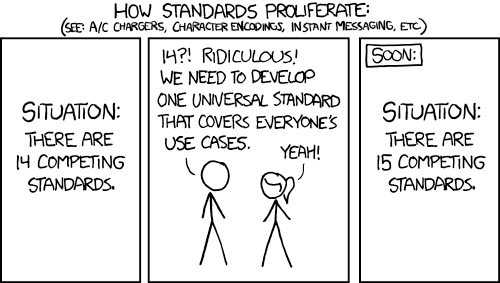
\includegraphics[width=\textwidth]{standards.png}
\end{center}
\end{frame}

\subsection{RGB Color Model}
\begin{frame}{RGB}
\begin{center}
  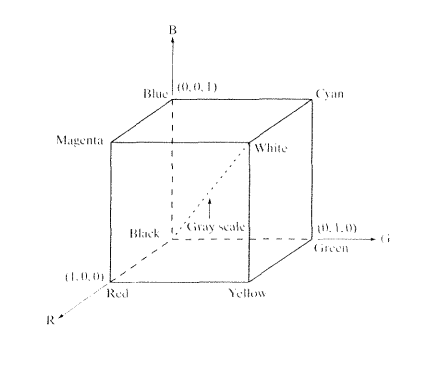
\includegraphics[width=\textwidth]{rgb.png}
\end{center}
\end{frame}

\subsection{CMY Color Model}
\begin{frame}{CMY(K)}
\[\begin{bmatrix}C\\M\\Y\end{bmatrix}
= \begin{bmatrix}1\\1\\1\end{bmatrix}
- \begin{bmatrix}R\\G\\B\end{bmatrix}\]
\begin{center}
  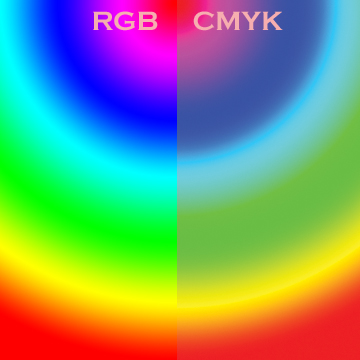
\includegraphics[width=0.5\textwidth]{rgb-vs-cmyk.jpg}
\end{center}
\end{frame}

\subsection{HSV Color Model}
\begin{frame}{HSV}
\begin{center}
  \includegraphics[width=\textwidth]{hsv.png}
\end{center}
\end{frame}

\begin{frame}[fragile]{BGR to HSV}
\begin{verbatim}
def bgr_to_hsv(b, g, r):
    minc, maxc = min(r, g, b), max(r, g, b)
    if minc == maxc: return 0.0, 0.0, maxc
    diff = maxc - minc
    sat = diff / maxc
    rc, gc, bc = (maxc-r)/diff, (maxc-g)/diff, ...
    if r == maxc: return (bc-gc)/6%1, sat, maxc
    if g == maxc: return (2.0+rc-bc)/6%1, sat, maxc
    if b == maxc: return (4.0+gc-rc)/6%1, sat, maxc
\end{verbatim}
\end{frame}

\begin{frame}[fragile]{HSV to BGR}
\begin{verbatim}
def hsv_to_bgr(h, s, v):
    if s == 0.0: return v, v, v
    f = h * 6 % 1
    p = v * (1 - s)
    q = v * (1 - s*f)
    t = v * (1 - s*(1 - f))
    i = int(h*6%6)
    if i == 0: return p, t, v
    if i == 1: return p, v, q
    if i == 2: return t, v, p
    if i == 3: return v, q, p
    if i == 4: return v, p, t
    if i == 5: return q, p, v
\end{verbatim}
\end{frame}

\begin{frame}[fragile]{Color Space Conversion}
\begin{verbatim}
from itertools import starmap
from numpy import reshape, uint8

def convert_color(image, func):
    x, y, z = image.shape
    return reshape(
        list(starmap(func, reshape(image, (x*y,z)))),
        (x, y, z)).astype(uint8)
\end{verbatim}

  \begin{itemize}
    \item \verb|func| takes range 0--255 instead of 0--1
    \item For \verb|@decorator| see source code
    \item Slow!  Better stick to \verb|cv2.cvtColor|
  \end{itemize}
\end{frame}

\section{Color Image Enhancements}
\frame{\tableofcontents[currentsection]}
\subsection{Chromatic Aberration Mitigation}
\begin{frame}{Chromatic Aberration}
  \begin{itemize}
    \item Often seen in pictures taken by cheap lenses
    \item Modern game devs love it
  \end{itemize}
  \begin{center}
    \includegraphics[width=0.5\textwidth]{ca4_before.png}
  \end{center}
\end{frame}

\begin{frame}{Mitigation}
  \begin{itemize}
    \item Mostly impossible to generalize (depend on lenses)
    \item Detection is easy though
  \end{itemize}
  \begin{center}
    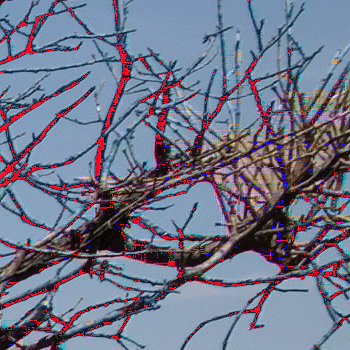
\includegraphics[width=0.5\textwidth]{ca4_detect.png}
  \end{center}
\end{frame}

\section{Pseudo Color Rendering}
\frame{\tableofcontents[currentsection]}
\begin{frame}{Pseudo Color Rendering}\Large
  \begin{itemize}
    \item Map grey intensity to color
    \item Get color image from greyscale image
    \item Enhance humans' visual intuition
    \item Common use: elevation,\\
      thermal, medical imaging
  \end{itemize}
\end{frame}

\begin{frame}[fragile]{Implementation}
\begin{verbatim}
from numpy import stack, vectorize

def map_color(grey, mapping):
    r = vectorize(lambda i: mapping[i][0])
    g = vectorize(lambda i: mapping[i][1])
    b = vectorize(lambda i: mapping[i][2])
    return stack((b(grey), g(grey), r(grey)), -1)
\end{verbatim}

\verb|cv2.applyColorMap| is still faster!
\end{frame}

\begin{frame}{Example: Elevation}
  \begin{center}
    \includegraphics[width=0.49\textwidth]{heightmap-grey.png}
    \includegraphics[width=0.49\textwidth]{heightmap-turbo.png}
  \end{center}
\end{frame}

\section{Conclusion}
\frame{\tableofcontents[currentsection]}
\begin{frame}{Copying}\Large
  \begin{center}
    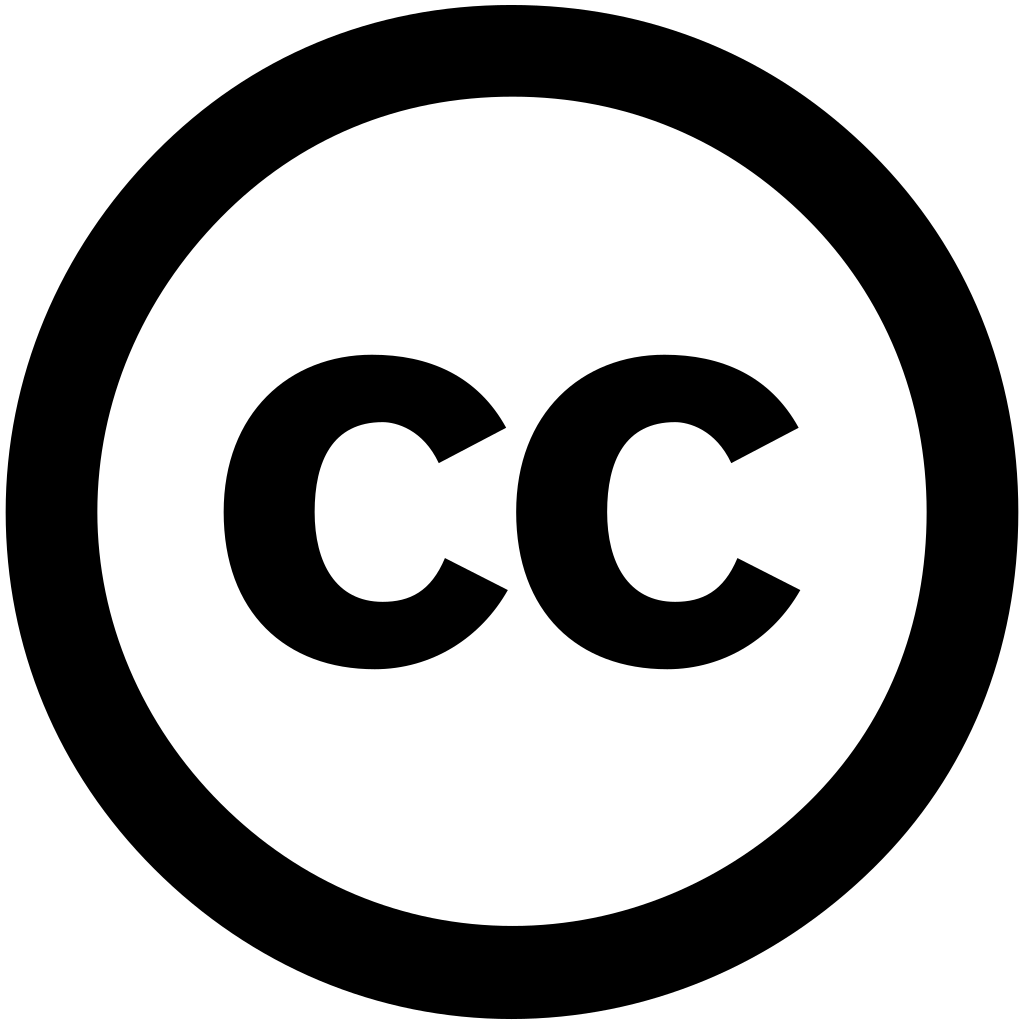
\includegraphics[width=0.2\textwidth]{CC.png}
    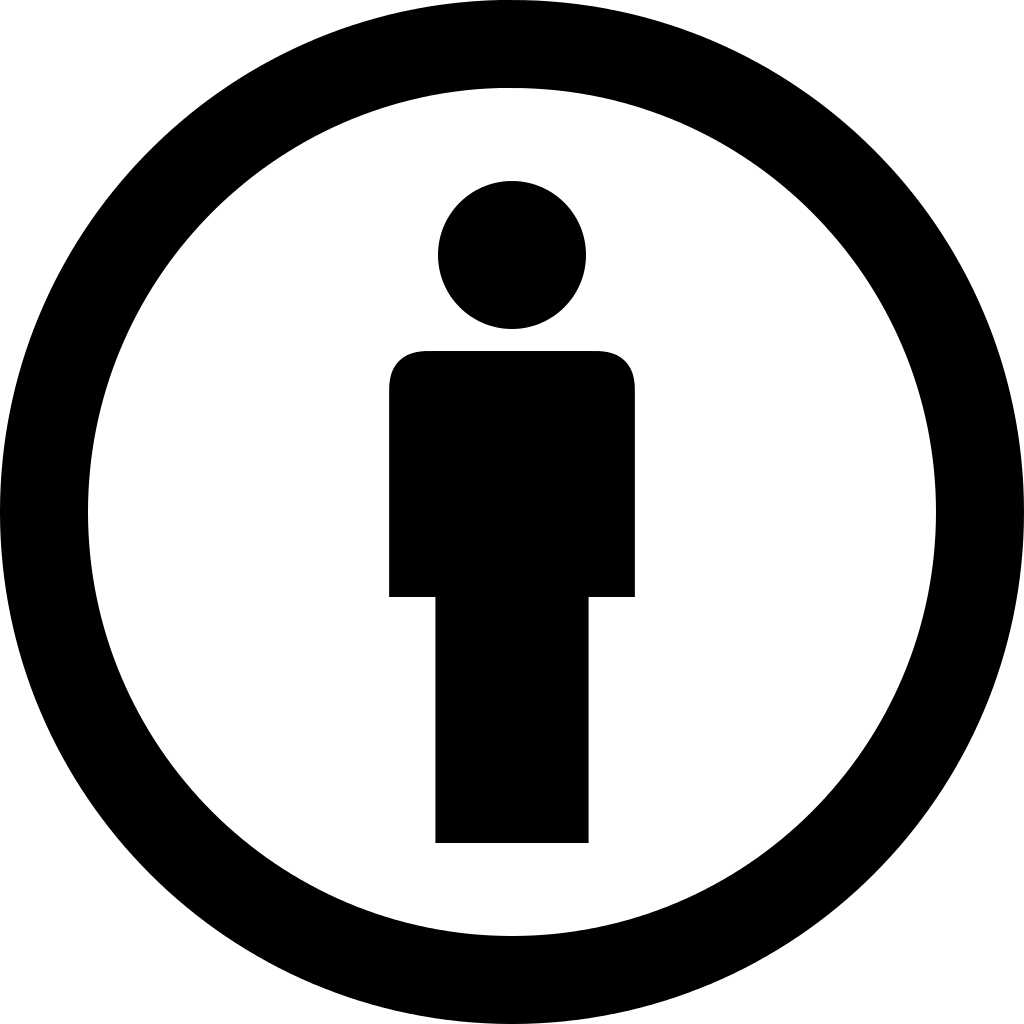
\includegraphics[width=0.2\textwidth]{BY.png}
    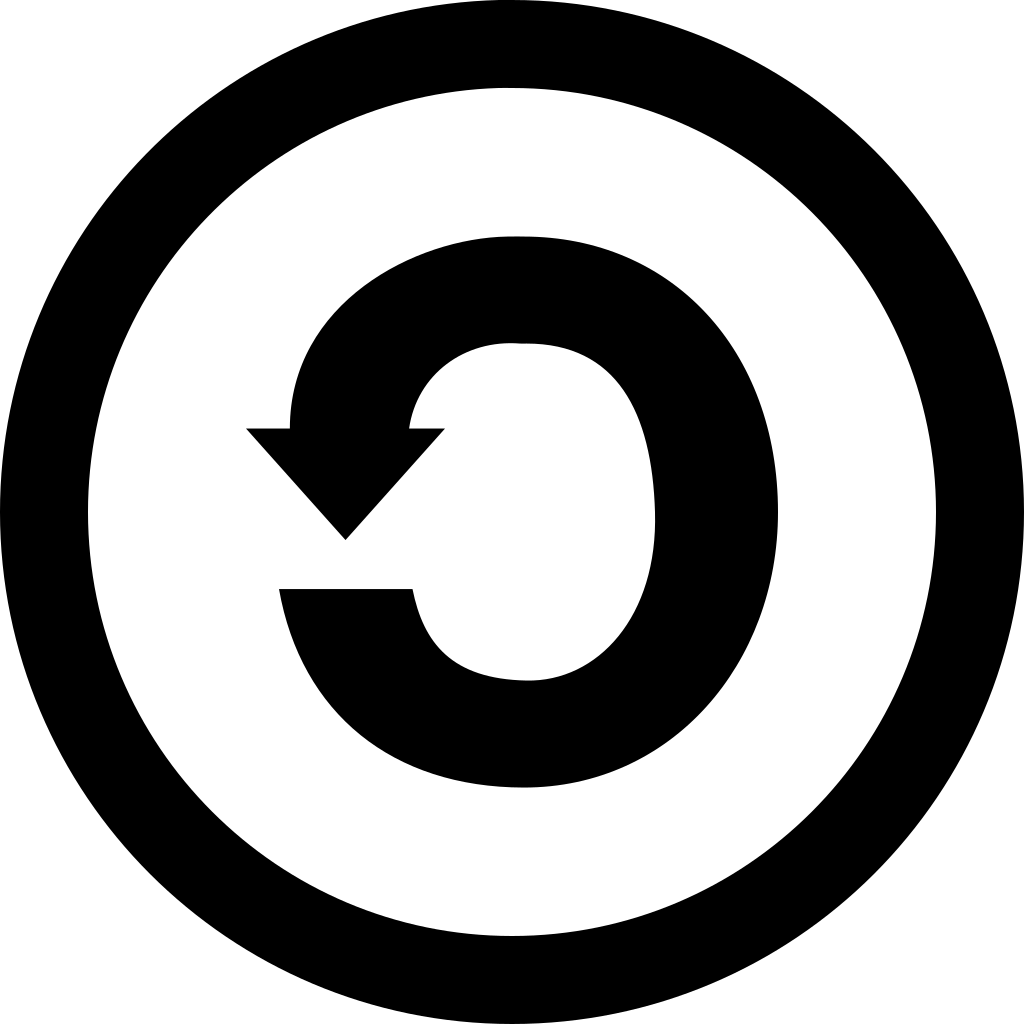
\includegraphics[width=0.2\textwidth]{SA.png}
  \end{center}

  This work is licensed under a
  \href{https://creativecommons.org/licenses/by-sa/4.0/}{Creative Commons
  Attribution-ShareAlike 4.0 International License}.
\end{frame}
\end{document}
